%%******************************************************************************
%%
%% pesqbib.tex
%%
%%******************************************************************************
%%
%% Title......: Introduction
%%
%% Author.....: GSCAR-DFKI
%%
%% Started....: Nov 2013
%%
%% Emails.....: renan028@gmail.com
%%
%% Address....: Universidade Federal do Rio de Janeiro
%%              Caixa Postal 68.504, CEP: 21.945-970
%%              Rio de Janeiro, RJ - Brasil.
%%
%%******************************************************************************


%%******************************************************************************
%% SECTION - Pesquisa Técnica
%%******************************************************************************
\setcounter{secnumdepth}{3}
\section{Pesquisa técnica e de fornecedores}
\label{pesqtec}

\subsection{Sensores}
A pesquisa técnica abordou os seguintes sistemas de sensoriamento: sensor de força, sensor indutivo de proximidade,
 sensor capacitivo de proximidade, sistema de atuação independente, sensor de
 campo magnético, sensoriamento por campo elétrico. Em sequência foi realizada a
 pesquisa por fornecedores que atendam aos requisitos de projeto.
 
\subsubsection{Sensor de força}

 Sensores de força podem ser utilizados para detectarem a presença da garra pescadora. A análise quantitativa e comparativa dessas forças pode indicar encaixe mal ou bem sucedido durante a operação e, portanto, é considerada uma solução viável mediante calibração. Os diversos tipos de sensores de força e suas aplicações podem ser consultados em \textbf{Guide to the Measurement of Force}, publicado por \textbf{The Institute of Measurement and Control, London}.

 O sensor de força é composto por um transdutor, que é submetido à força, e uma instrumentação associada, responsável por alimentar o transdutor e processar a saída. O transdutor é um dispositivo que recebe um estímulo físico, como a contração elástica do material devido ao peso, e traduz em outra medida física, como variação de voltagem ou corrente elétrica. Esta variação obedece uma relação conhecida e, dessa forma, é possível determinar quantitativamente a força aplicada.

 Existem diversos sensores de força disponíveis no mercado, com sistemas variados de operação. As principais características a serem consideradas na escolha de um sensor de força são: curva de resposta, capacidade máxima, não-linearidade, histerese, sensibilidade e reprodutibilidade.

 O sensor de força mais utilizado e que atende aos requisitos do projeto é o strain gauge. A força atua em um metal cilíndrico, que é comprimido e altera a resistência de um strain gauge, acoplado à superfície do cilindro (ver figura~\ref{forca_1}).

 \begin{figure}[H]
    \centering
    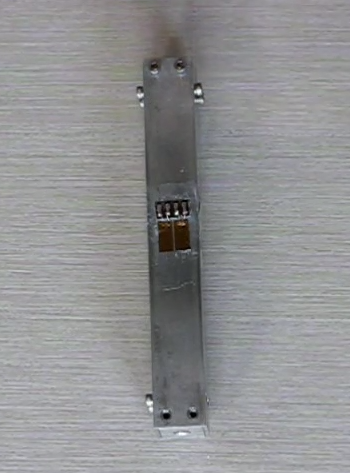
\includegraphics[width=0.4\columnwidth]{figs/forca/1.png}
    \caption{Exemplo de um sensor de força: cilindro com strain gauge acoplado.}
    \label{forca_1}
\end{figure}


 A resistência elétrica de um fio varia conforme seu comprimento e sua área, portanto, a variação de corrente que passa por este fio pode ser utilizada como medida quantitativa e é possível determinar a força aplicada por um modelo matemático conhecido: $R=\frac{\rho L}{A}$. Outros sensores que poderiam atender às especificações, mas são de mais difícil comercialização, em relação aos requisitos de projeto, são: sensor de força piezoelétrico

 De acordo com \textbf{Guide to the Measurement of Force}, a aplicação pode ser caracterizada como sistema para medições e controle de forças para operações de segurança. Pode ainda ser especificada como \textbf{Crane overload/underload protection}, que consiste em monitorar forças atuando em garras tipo pescadora ou gancho (ver figura~\ref{forca_2}), no qual a medida será avaliada em situações estáticas ou de pouco movimento/vibração.

  \begin{figure}[H]
    \centering
    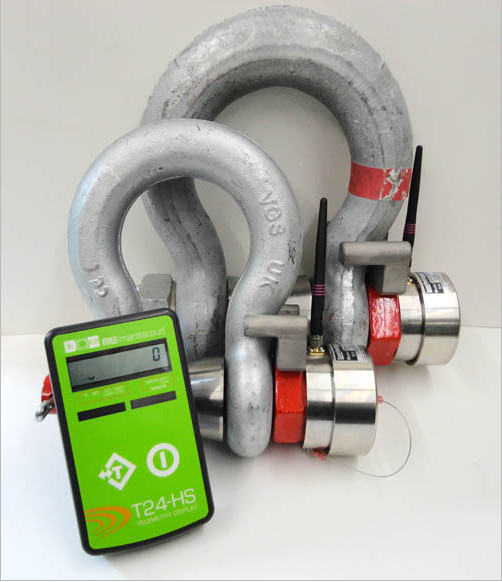
\includegraphics[width=0.4\columnwidth]{figs/forca/2.png}
    \caption{Exemplo de instalação de sensor de força em garra.}
    \label{forca_2}
\end{figure}

 \paragraph{Conclusão de análise técnica}\mbox{}\\

A solução por sensores de força é eficiente em aplicações onde se deseja avaliar frequência de vibração e duração da onda de choque, porém não muito na medida quantitativa e comparativa de forças devido à sensibilidade do strain gauge a campos magnéticos externos, pressão hidrostática e umidade. A variação de acúmulo de sedimentos no stoplog também dificulta a calibração do instrumento.

 \paragraph{Pesquisa de fornecedores}\mbox{}\\

Os fornecedores para sensores de força do tipo strain gauge avaliados nesta pesquisa são: Applied Measurements Limited, Load Cell Central, Transducer Techniques. Os modelos avaliados são da série DBEP e CLP de seus respectivos fornecedores.

\subsubsection{Sensor indutivo de proximidade}

Sensores indutivos de proximidade podem ser utilizados para detectarem a presença da garra pescadora. Este sensor de presença pode ser do tipo linear, podendo ser realizada análise quantitativa, ou simplesmente chaveado, um simples indicador de presença. Portanto, pode indicar encaixe mal ou bem sucedido durante a operação de remoção/inserção de stoplogs. Os sensores indutivos apresentam a mesma forma de operação nos diversos produtos disponíveis no mercado, diferenciando-se principalmente na medida de distância da aplicação.

 O sistema para sensoriamento por indução magnética é composto por uma fonte de alimentação e um indutor. Ao alimentar o sensor indutivo, uma corrente alternada é gerada. A corrente elétrica que passa pelo indutor gera um campo magnético na face do sensor. Este campo magnético induz corrente de Foucault no alvo metálico, que aumenta conforme o alvo se aproxima do sensor indutivo. O aumento das correntes de Foucault cria um campo magnético no alvo, que irá se opor ao campo produzido pelo sensor indutivo. Essa redução do campo magnético pode ser medida e, portanto, é possível presenciar o alvo.

 Existem diversos sensores indutivos disponíveis no mercado que atendem às especificações, apresentam o mesmo modo de operação e diferenciam-se principalmente quanto à robustez, instalação (faceada ou não) e interface de saída. A resistência a choques, vibração, submersibilidade e o tipo de instalação são as características mais importantes para a aplicação. O sensor deve ser do tipo IP69K e faceado, o que diminui o alcance, mas aumenta a proteção.

 A pesquisa por sensores indutivos de proximidade para a finalidade desejada resultou em aplicações equivalentes. A empresa \textbf{HATCH - Energy Innovations} desenvolveu em 2007 um Lifting Beam instrumentado com sensores indutivos (ver figura~\ref{indutivo_1}). Em 2008, a empresa \textbf{Atlas Polar} adotou a mesma solução com sensores indutivos.

 \begin{figure}[H]
    \centering
    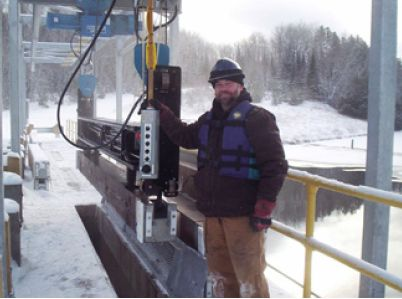
\includegraphics[width=0.5\columnwidth]{figs/indutivo/1.jpg}
    \caption{Lifting Beam desenvolvido pela empresa HATCH}
    \label{indutivo_1}
\end{figure}

 \paragraph{Conclusão de análise técnica}\mbox{}\\
A solução por sensores indutivos é eficiente em aplicações onde se deseja avaliar a presença de stoplog. A grande maioria dos sensores são frágeis a choque e vibração, além de sensíveis a ruídos elétricos e magnéticos. Porém, já há no mercado produtos IP69K e encapsulados. Há, também, a possibilidade de falso positivo em caso de sedimentos metálicos, mas é baixa a probabilidade.
Pesquisas em aplicações semelhantes mostraram que o sensor indutivo é a solução adotada para o monitoramento de encaixe entre garra pescadora e stoplog, auxiliado por outros sensores ou sistemas independentes de atuadores.

 \paragraph{Pesquisa de fornecedores}\mbox{}\\

Os fornecedores pesquisados para sensores indutivos que atendem aos requisitos de projeto são: Contrinex, Pepperl-Fuchs, Positek e Turck. Diversos modelos foram avaliados, juntamente com os técnicos das respectivas empresas.
As vantagens apresentadas e a utilização desse tipo de sensoriamento em
aplicações equivalentes foram decisivos para a escolha por esta solução em nossa
aplicação. O modelo selecionado, após ampla análise entre fornecedores, é o
modelo NBB20-L2-E2-V1 de instalação faceada, chaveado normalmente aberto e
distância de operação de 2cm (figura~\ref{indutivo_1}).

\begin{figure}[H]
    \centering
    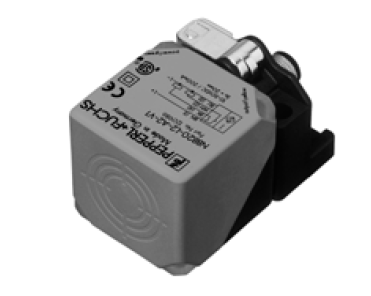
\includegraphics[width=0.4\columnwidth]{figs/indutivo/1.png}
    \caption{Sensor indutivo do fornecedor Pepperl-Fuchs.}
    \label{indutivo_1}
\end{figure}

\subsubsection{Sensor capacitivo de proximidade}
Os sensores capacitivos de proximidade são capazes de detectar objetos devido à capacidade destes alvos em serem carregados eletricamente. Analogamente ao sensor indutivo, que detecta variações de campo magnético devido a alvos metálicos, o sensor capacitivo é sensível a variações na capacitância (ver figura~\ref{capacitivo_1}).

\begin{figure}[H]
    \centering
    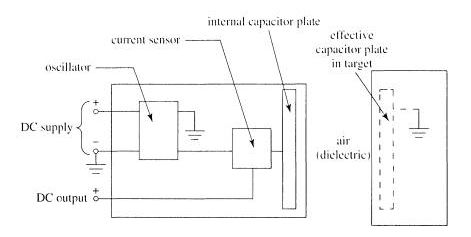
\includegraphics[width=0.8\columnwidth]{figs/capacitivo/1.jpg}
    \caption{Sensor capacitivo}
    \label{capacitivo_1}
\end{figure}

Internamente ao sensor, há um circuito que utliza a alimentação DC para gerar voltagem alternada (oscilador). O circuito interno RC é, então, alimentado e uma corrente alternada passa por esse circuito. O fluxo de corrente alternada depende da capacitância, e esta varia  conforme a distância e área entre as placas do capacitor e o material dielétrico entre as placas: $C = \frac{\epsilon A}{d}$.

Em sensores capacitivos, uma placa do capacitor está no sensor e a outra é o objeto a ser detectado, que pode ser um material metálico ou não-metálico. A aproximação do alvo modifica a capacitância, resultando em variações no campo elétrico e na corrente alternada. Finalmente, as variações da corrente podem ser medidas e o alvo é detectado.

As características que devem ser avaliadas em sensores capacitivos são as mesmas dos sensores indutivos, como tipo de instalação, modo de operação chaveado ou linear e etc. Porém, deve-se atentar ao fator de redução, que depende do alvo a ser detectado.

 \paragraph{Conclusão de análise técnica}\mbox{}\\
 Os sensores capacitvos exercem função semelhante ao sensor indutivo e pode ser utilizado para detecção de presença de stoplog. Porém, a calibração se mostra bem mais complexa devido à sensibilidade do sensor e ao fato de não estar restrito a detecção de materiais metálicos. A chance de falsos positivos será bem maior em caso de escolha deste sensor em comparação com o sensor indutivo.
 \paragraph{Pesquisa de fornecedores}\mbox{}\\
Os fornecedores pesquisados de sensores capacitivos são os mesmos fornecedores de sensores indutivos.

\subsubsection{Encoder}
O Sistema de Lifting Beam desenvolvido em aplicação semelhante de remoção e inserção de stoplogs pela empresa \textbf{HATCH} utliza atuadores elétricos independentes em cada garra, o que permite o monitoramento da abertura das garras, sendo possível saber quando há encaixe mal ou bem sucedido. O sistema em estudo a ser desenvolvido, porém, é um Lifting Beam mecânico, onde as garras abrem e fecham passivamente conforme o Lifting Beam é atuado e a chave de operação é selecionada em uma determinada posição. Por questões de restrição de projeto, não é permitido alterar a estrutura mecânica de forma que as garras sejam atuadas independentemente, mas é permitida a instrumentação do Lifting Beam com encoders, sendo possível instalá-los nas vigas das garras, a fim de medir suas posições angulares.A movimentação angular das garras durante o encaixe é conhecido e sequencial, de forma que uma simples anlálise comparativa com os dados fornecidos pelos encoders durante a execução da tarefa pode indicar se o encaixe foi mal ou bem sucedido.

O encoder óptico é um dispositivo eletromecânico que entrega como saída um sinal elétrico proporcional à posição angular do eixo acoplado. O eixo é acoplado mecanicamente a um disco opaco e marcado em sua superfície por segmentos (ver figura~\ref{encoder_1}).

\begin{figure}[H]
    \centering
    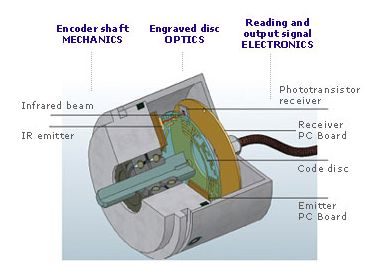
\includegraphics[width=0.5\columnwidth]{figs/encoder/1.jpg}
    \caption{Sistema interno de um encoder.}
    \label{encoder_1}
\end{figure}

Diodos emissores de luz infravermelha alcança os receptores através das fendas do disco. O sinal analógico é criado, amplificado, convertido em digital e transmitido ao processador.

Além dos requisitos básicos do projeto, como submersibilidade e resistência a choque e vibração, as principais características a serem avaliadas neste projeto para a escolha de um encoder são: modo de operação incremental ou absoluto, multi-voltas ou não, interface de comunicação, resolução e tensão de operação.

 \paragraph{Conclusão de análise técnica}\mbox{}\\
A pesquisa mostrou ampla aplicação de encoders para a aplicação e é esperado que seja possível identificar encaixe mal ou bem sucedido com sua utilização. A instalação do encoder na viga da garra pescadora não é mecanicamente complexa e não resultará em alteração permanente da estrutura.

 \paragraph{Pesquisa de fornecedores}\mbox{}\\
Os fornecedores para encoders que atendem aos requisitos de projeto pesquisados são: Hohner, IFM, Pepperl-Fuchs e Rotary Encoder Solutions.

As vantagens apresentadas e a utilização desse tipo de sensoriamento em
aplicações equivalentes foram decisivos para a escolha por esta solução em nossa
aplicação. O modelo selecionado, após ampla análise entre fornecedores, é o
modelo Encoder RM9000 Absoluto com interface CAN, multi-voltas.
(figura~\ref{encoder_1})

\begin{figure}[H]
    \centering
    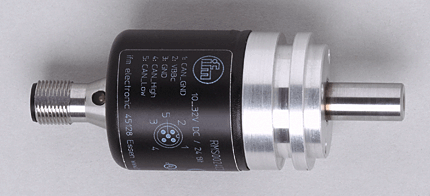
\includegraphics[width=0.4\columnwidth]{figs/encoder/1.png}
    \caption{Encoder do fornecerdor IFM}
    \label{encoder_1}
\end{figure}

\subsubsection{Sensor de campo magnético}
O stoplog é um bloco metálico e esta característica física pode ser aproveitada em soluções de circuito magnético e elétrico.

Um circuito magnético consiste em uma malha fechada que contém um fluxo magnético através de condutores. A solução estudada é induzir um campo magnético em uma garra e utilizar um sensor de campo magnético na outra extremidade do Lifting Beam, fazendo com que o próprio stoplog seja o condutor. A permeabilidade magnética do stoplog é maior do que a permeabilidade da água e, dessa forma, o sensor de cmapo magnético detectaria variações no caso de presença de stoplog. (ver figura~\ref{magnetico_1})

\begin{figure}[H]
    \centering
    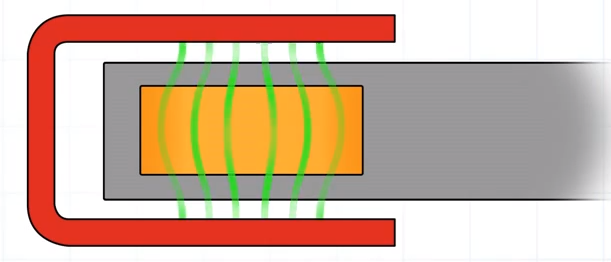
\includegraphics[width=0.5\columnwidth]{figs/magnetico/1.png}
    \caption{Circuito magnético.}
    \label{magnetico_1}
\end{figure}


 \paragraph{Conclusão de análise técnica}\mbox{}\\
Sensores magnéticos exigem uma área de pouca interferência magnética, são muito sensíveis e necessitam de calibração rigorosa para cada aplicação. Além disso, a distância entre gerador de campo e sensor é longa devido ao comprimento do stoplog, o que exige ainda maior sensibilidade do sensor e grandes geradores. Esta solução não foi selecionada.

\subsubsection{Sensoriamento por campo elétrico}
Outra solução semelhante ao circuito magnético e que utiliza a vantagem da propriedade física metálica do stoplog é o circuito elétrico.

O circuito elétrico é formado por uma diferença de potencial entre dois terminais em uma malha fechada. Na aplicação, o stoplog fecha a malha do circuito e será equivalente a uma resistência e pode ser realizada tanto a configuração de divisor de tensão, como a medição da corrente por efeito hall (~\ref{senseletrico_1}).

\begin{figure}[H]
    \centering
    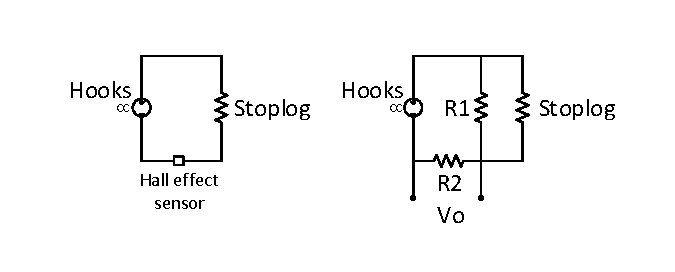
\includegraphics[width=1\columnwidth]{figs/senseletrico/1.pdf}
    \caption{Circuito elétrico}
    \label{senseletrico_1}
\end{figure}


 \paragraph{Conclusão de análise técnica}\mbox{}\\
 A solução apresentada, apesar de eficaz, apenas indica a presença de stoplog, não o encaixe mal ou bem sucedido. Além disso, há grande possibilidade de sedimentos e ferrugem prejudicarem no sensoriamento do sistema. Esta solução não foi selecionada.

\subsubsection{Sonar}
Sonar\footnote{A sigla tem origem como acrônimo de \textit{sound navigation and ranging}.} é uma técnica que utiliza a propagação do som na água para se comunicar e detectar objetos nesse meio, ela possui duas vertentes uma chamada ativa e outra passiva. A passiva se resume a escutar o meio e não será investigada, pois não possui a funcionalidade para o mapeamento de superfícies submersas. Os equipamentos que fazem uso de tal tecnologia acabam por herdar seu nome, assim sonares que utilizam a tecnologia ativa são chamados de sonares ativos.

O sonar ativo, daqui em diante apenas referido como sonar, emite um ping que é um pulso de onda sonora que será refletido pelo meio. Conforme a frente de onda atravessa os objetos submersos ela é refletida e este eco é detectado no retorno pelo sonar, onde ele extrai as informações do tempo que a onda levou para retornar e sua intensidade, podendo, a partir do conhecimento de características do meio, como a velocidade de propagação do som, estimar a distancia de origem do eco e consequentemente do objeto.

Pela aplicação os sonares são divididos em basicamente duas categorias: \emph{profiling} e \emph{imaging};

O sonar do tipo \emph{imaging} são tipicamente utilizados para fazer o mapeamento do fundo do mar, possuindo uma abertura em formato de leque (ver figura~\ref{sonar_1}), eles podem utilizar um motor de rotação sobre o eixo perpendicular ao feixe ou podem ser arrastados pela água para fazer o escaneamento (ver figura~\ref{sonar_2}).

\begin{figure}[H]
    \centering
    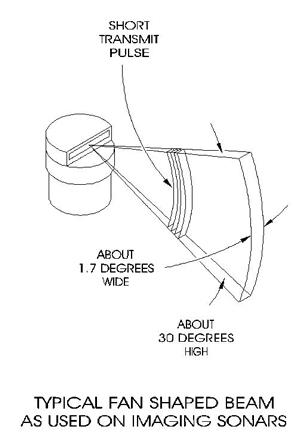
\includegraphics[width=0.5\columnwidth]{figs/sonar/1.jpg}
    \caption{Típico feixe em formato de leque de sonares tipo \emph{imaging}}
    \label{sonar_1}
\end{figure}

\begin{figure}[H]
    \centering
    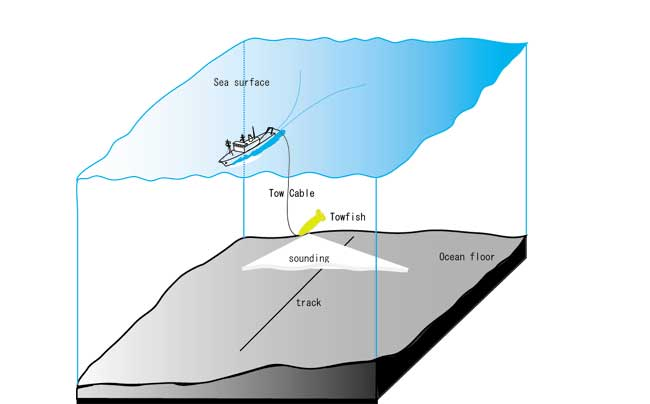
\includegraphics[width=0.5\columnwidth]{figs/sonar/2.jpg}
    \caption{Sonar \emph{imaging} sendo arrastado para mapeamento das profundezas}
    \label{sonar_2}
\end{figure}


A resposta dos sonares tipo \emph{imaging} forma uma imagem colorida exibindo tons diferentes para respostas mais fortes e mais fracas de eco do sonar. Sendo utilizado para obter uma imagem do fundo do mar semelhante as que os radares fazem na superfície.

Pela tecnologia empregada os sonares \emph{imaging} possuem dois tipos de configuração: \emph{multibeam} e \emph{mechanical} (single beam).

A configuração \emph{single beam} possui um transdutor acoplado a um mecanismo de \emph{pan} para possibilitar a varredura de determinada área. Assim, o sonar envia seu \emph{ping} espera o eco de retorno e avança para a próxima posição determinada pelo passo, ou resolução angular, do motor que compõe o mecanismo de \emph{pan}.

Alternativamente, os sonares \emph{multibeam} possuem idealmente um feixe \emph{ping} extremamente amplo, sendo na prática composto por diversos feixes com seus respectivos transdutores sincronizados. Essa configuração possui diversos receptores espalhados por uma região do sonar, resolvendo qual a posição de origem do eco através de um sistema de multilateração. Assim, o \emph{multibeam} sobrepuja a configuração \emph{single beam} no aspecto de precisão e tempo de varredura.

De forma diferente, os sonares do tipo \emph{profiling} retornam apenas um valor e não uma graduação de tons. Esse valor é referente, normalmente, ao tempo de retorno do eco mais intenso dentro do intervalo de amostragem, intervalo de espera que delimita o alcance máximo de interesse. Esses sonares também podem ser configurados para enviarem o valor do tempo de retorno do primeiro eco, em vez do mais intenso, de maneira a agilizar o processo de captura de dados, pois todos os ecos à partir do primeiro são ignorados, passando para a emissão de um novo \emph{ping} em uma nova posição.

Outra característica importante dos sonares \emph{profiling} é o formato do seu feixe, este possui uma abertura estreita de formato tipicamente cônico (ver figura~\ref{sonar_3}).

\begin{figure}[H]
    \centering
    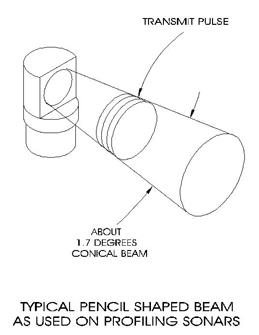
\includegraphics[width=0.5\columnwidth]{figs/sonar/3.jpg}
    \caption{Típico feixe em formato de cone de sonares tipo \emph{profiling}}
    \label{sonar_3}
\end{figure}



 \paragraph{Conclusão de análise técnica}\mbox{}\\
 O ambiente no qual será utilizado o sonar possui uma profundidade inferior a 20
 metros e a necessidade de mapeamento se localiza sobretudo em uma área de
 aproximadamente $2 \times 15 m^2$. Para essa situação o sonar profiling se
 mostra como o mais apropriado devido ao seu estreito feixe que otimiza a
 precisão para uma pequena superfície pouco profunda.
 \paragraph{Pesquisa de fornecedores}\mbox{}\\
 Os fornecedores para sonares avaliados nesta pesquisa são: Blueview, Echoscope,
 Marine Solution e Tritech. O modelo escolhido é o Super SeaKing DFP da Tritech.


\subsection{Reconstrução de superfície 3D}

Muitos dos problemas encontrados na operação de inserção e remoção dos
\textit{stoplogs} são provenientes da existência de objetos estranhos, trazidos
pelo próprio rio, presentes no leito de concreto ou na superfície de um dos
\textit{stoplogs}. A inspeção da existência de tais objetos, isto é, a sua
visualização, é de suma importância para que se possa determinar corretamente
qual ação corretiva é a mais apropriada.

Em ambientes subaquáticos onde o meio possui uma boa visibilidade, é possível a
utilização de câmeras para a realização da inspeção. Porém em ambientes onde a
visibilidade não é satisfatória, a utilização de câmeras fica inviabilizada.
Para esses casos, é necessário a utilização de outros métodos e sensores para a
visualização do ambiente a ser inspecionado. Porém os sensores utilizados para
mapear os ambientes não tem uma resposta que é facilmente interpretada pelo ser
humano e, por isso, é necessário que se faça uma conversão dos dados e uma a
construção de uma representação 3D da superfície.

Uma reconstrução 3D de superfície consiste na interpretação e combinação de
dados, afim de se extrair informações tridimensionais do ambiente. Em ambientes
subaquáticos com pouca visibilidade, o sensor recomendado para esse tipo de
operação é o sonar. A figura \ref{figs/3d/3dcomporta} exemplifica uma
reconstrução 3D obtida pelo processamento de dados provenientes de um sonar.
\begin{figure}[H]
    \centering 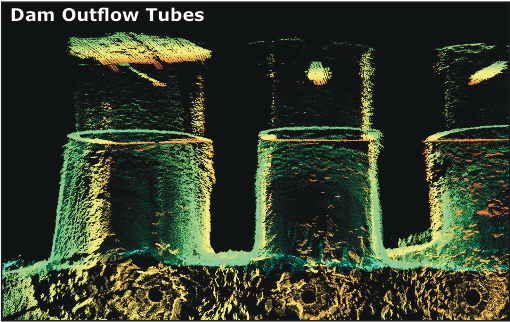
\includegraphics[width=0.9\textwidth]{figs/3d/3dcomporta}
    \caption{Exemplo de uma reconstrução 3D da sáida de uma barragem dos dados obtidos de um sonar 3D.}
    \label{figs/3d/3dcomporta}
\end{figure}


Um dos pontos determinantes para uma boa reconstrução 3D é a forma de se representar e armazenar as informações tridimensionais, já interpretadas dos sensores. Uma boa representação 3D deve possuir uma boa fidelidade do ambiente real representado, ter boa velocidade de processamento e pouca utilização de memória do sistema.

Após a revisão bibliográfica realizada, os tipos de armazenamento e representação mais recentes e avançados existentes na literatura eram a representação a partir de pointclouds, mapas de elevação e octomaps. A representação escolhida foi a por meio de octomaps. A seguir será realizado uma descrição das principais característica de cada método.
\begin{itemize}
    \item \textbf{Pointcloud} - Armazena as coordenadas tridimensionais de cada ponto lido pelo sensor. Possui uma boa fidelidade de representação de ambientes 3D complexos, porém não é capaz de distinguir entre espaçoes vazios e ocupados.

    Por amazenar informações ponto a ponto, não possui uma eficiente utilização de memória. A figura \ref{fig:pointcloud} mostra a representação utilizando pointcloud de uma área externa.

    \begin{figure}[H]
    \centering
    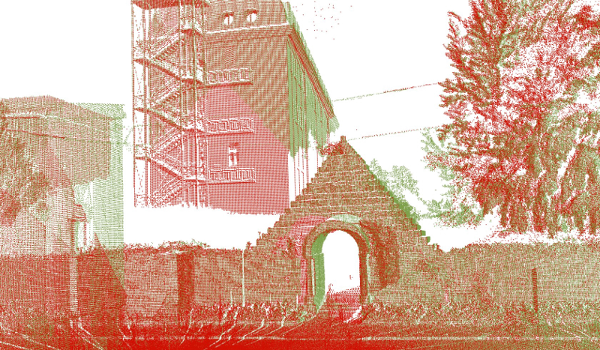
\includegraphics[width=0.8\textwidth]{figs/3d/registration_closeup}
    \caption{Exemplo de uma reconstrução tridimensional representado por uma Pointcloud}
    \label{fig:pointcloud}
\end{figure}


    \item \textbf{Mapas de elevação} - Os mapas de elevação representam uma superfície através de um grid 2D e armazenam uma informação de elevação para cada célula. Os mapas de elevação tem uma melhor eficiência de memória, porém para atingir essa virtude perdem o poder de representação fiel em todas as dimensões. A figura \ref{fig:elevacao} mostra a representação utilizando mapas de elevação de uma área externa.

    \begin{figure}[H]
    \centering
    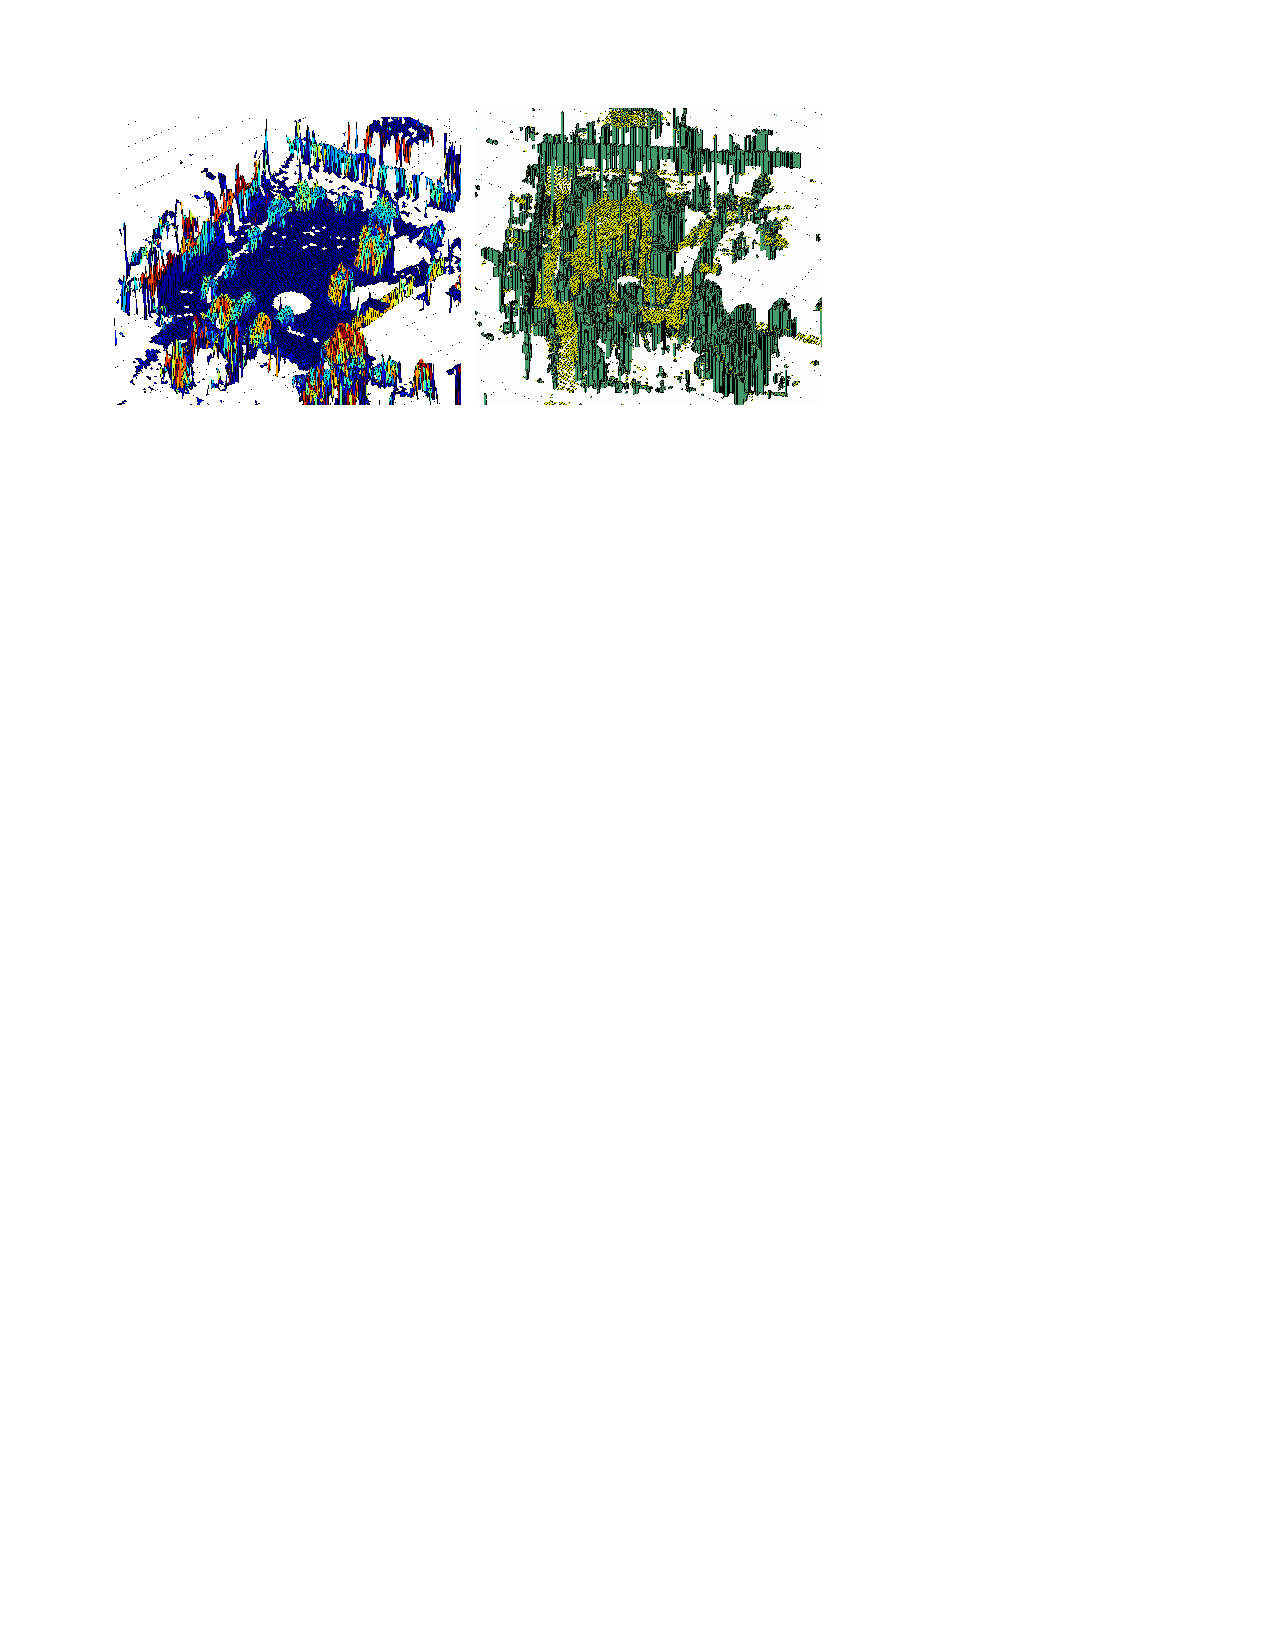
\includegraphics[width=0.8\textwidth]{figs/3d/elevationmap}
    \caption{Exemplo de uma reconstrução tridimensional representado por um Mapa de Elevação}
    \label{fig:elevacao}
\end{figure}

    \item \textbf{Octomap} - Octomap é um framework livre para mapeamento 3D baseado em uma estrutura hierárquica árvore de dados, chamada OcTree. O espaço tridimensional é recursivamente dividido em octantes, como exemplificado na figura \ref{fig:octree}. Aliada à estrutura de árvore, essa característica possibilita que somente a coordenada do ponto raiz do mapa necessite ser armazenada e todas as coordenadas dos demais pontos são inferidas através da posição relativa ao ponto raiz. Diminuindo, assim, a utilização de memória do sistema. A estrutura hierárquica possibilita, também, que no mapa gerado seja realizada buscas, segmentações para a análise separada de diferentes objetos e múltiplas resoluções, diferentemente de mapas de resolução fixa como no caso da representação com pointclouds.

    \begin{figure}[h!]
    \centering
    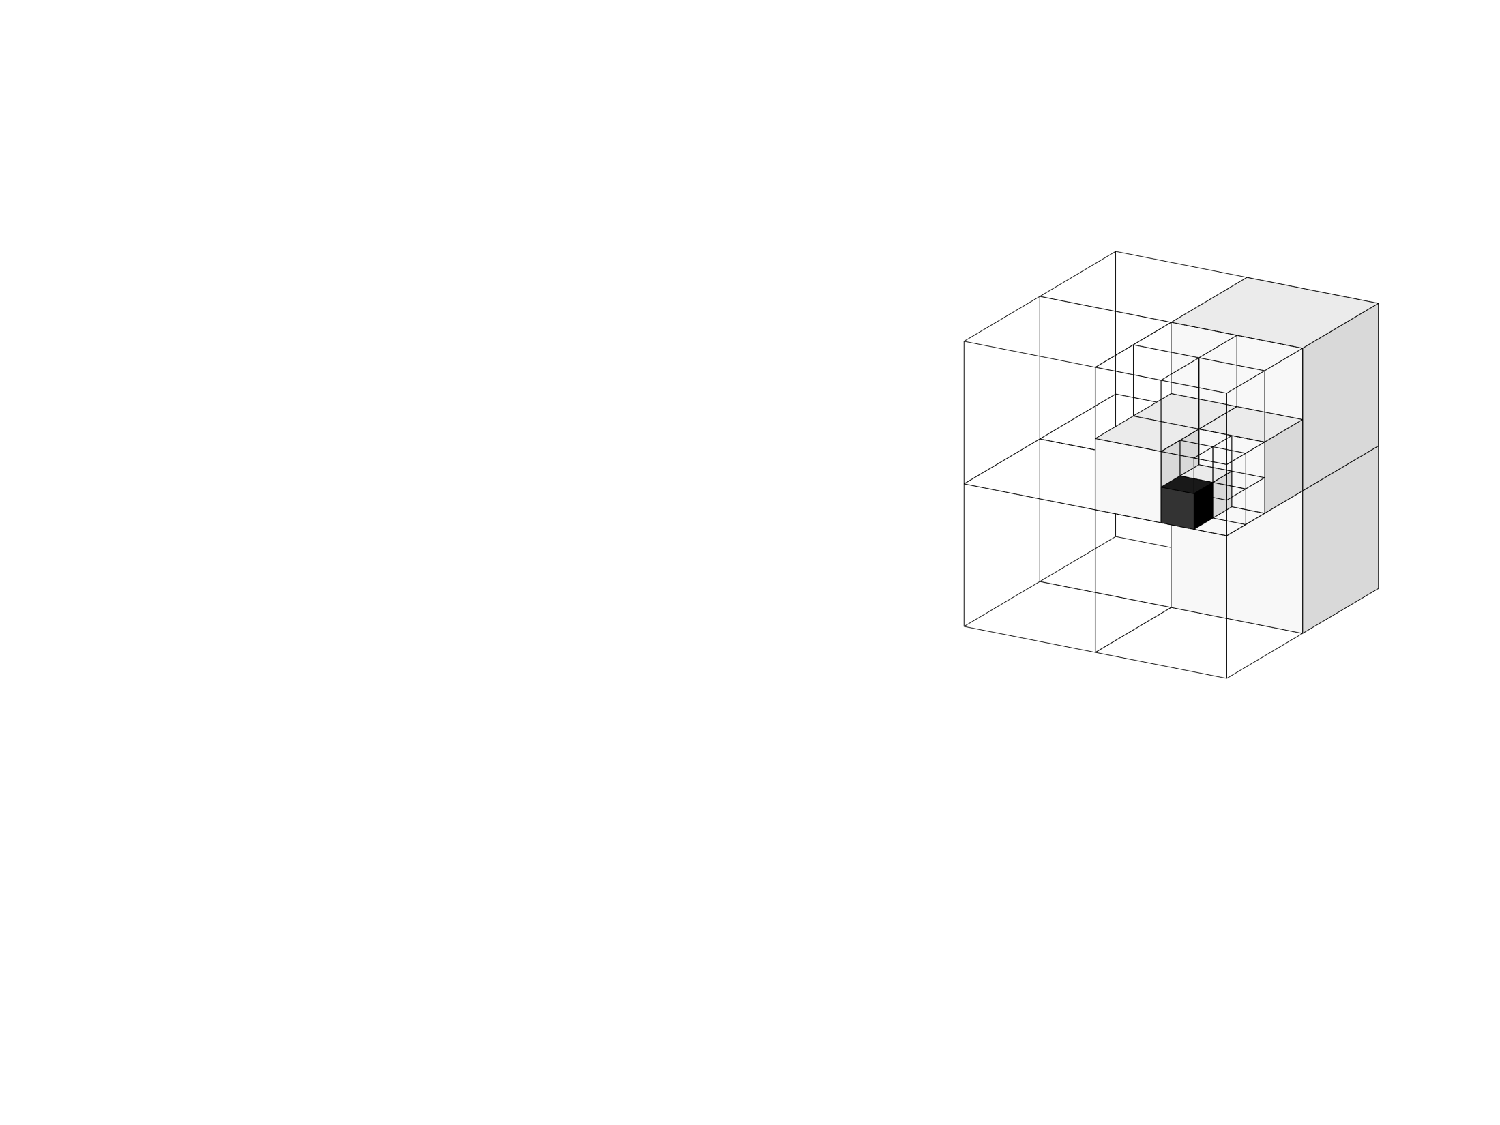
\includegraphics[width=0.4\textwidth]{figs/3d/octree}
    \caption{Divisão recursiva do espaço em octantes}
    \label{fig:octree}
\end{figure}
    O framework utiliza uma política de ocupância probabilística, o que possibilita uma boa caracterização de ambientes dinâmicos e atenuação de ruídos provenientes dos sensores. Outra vantagem importante é a diferenciação de espaços ocupados, vazios e desconhecidos, funcionalidade que não está presente em nenhum dos métodos já apresentados. A distinção entre espaços que estão desocupados e espaços ainda não explorados pelo sistema  pode ser visualizada na figura \ref{fig:free} e também uma comparação com a utilização de pointclouds para o mapeamento do mesmo ambiente.

    \begin{figure}[h!]
     \centering
    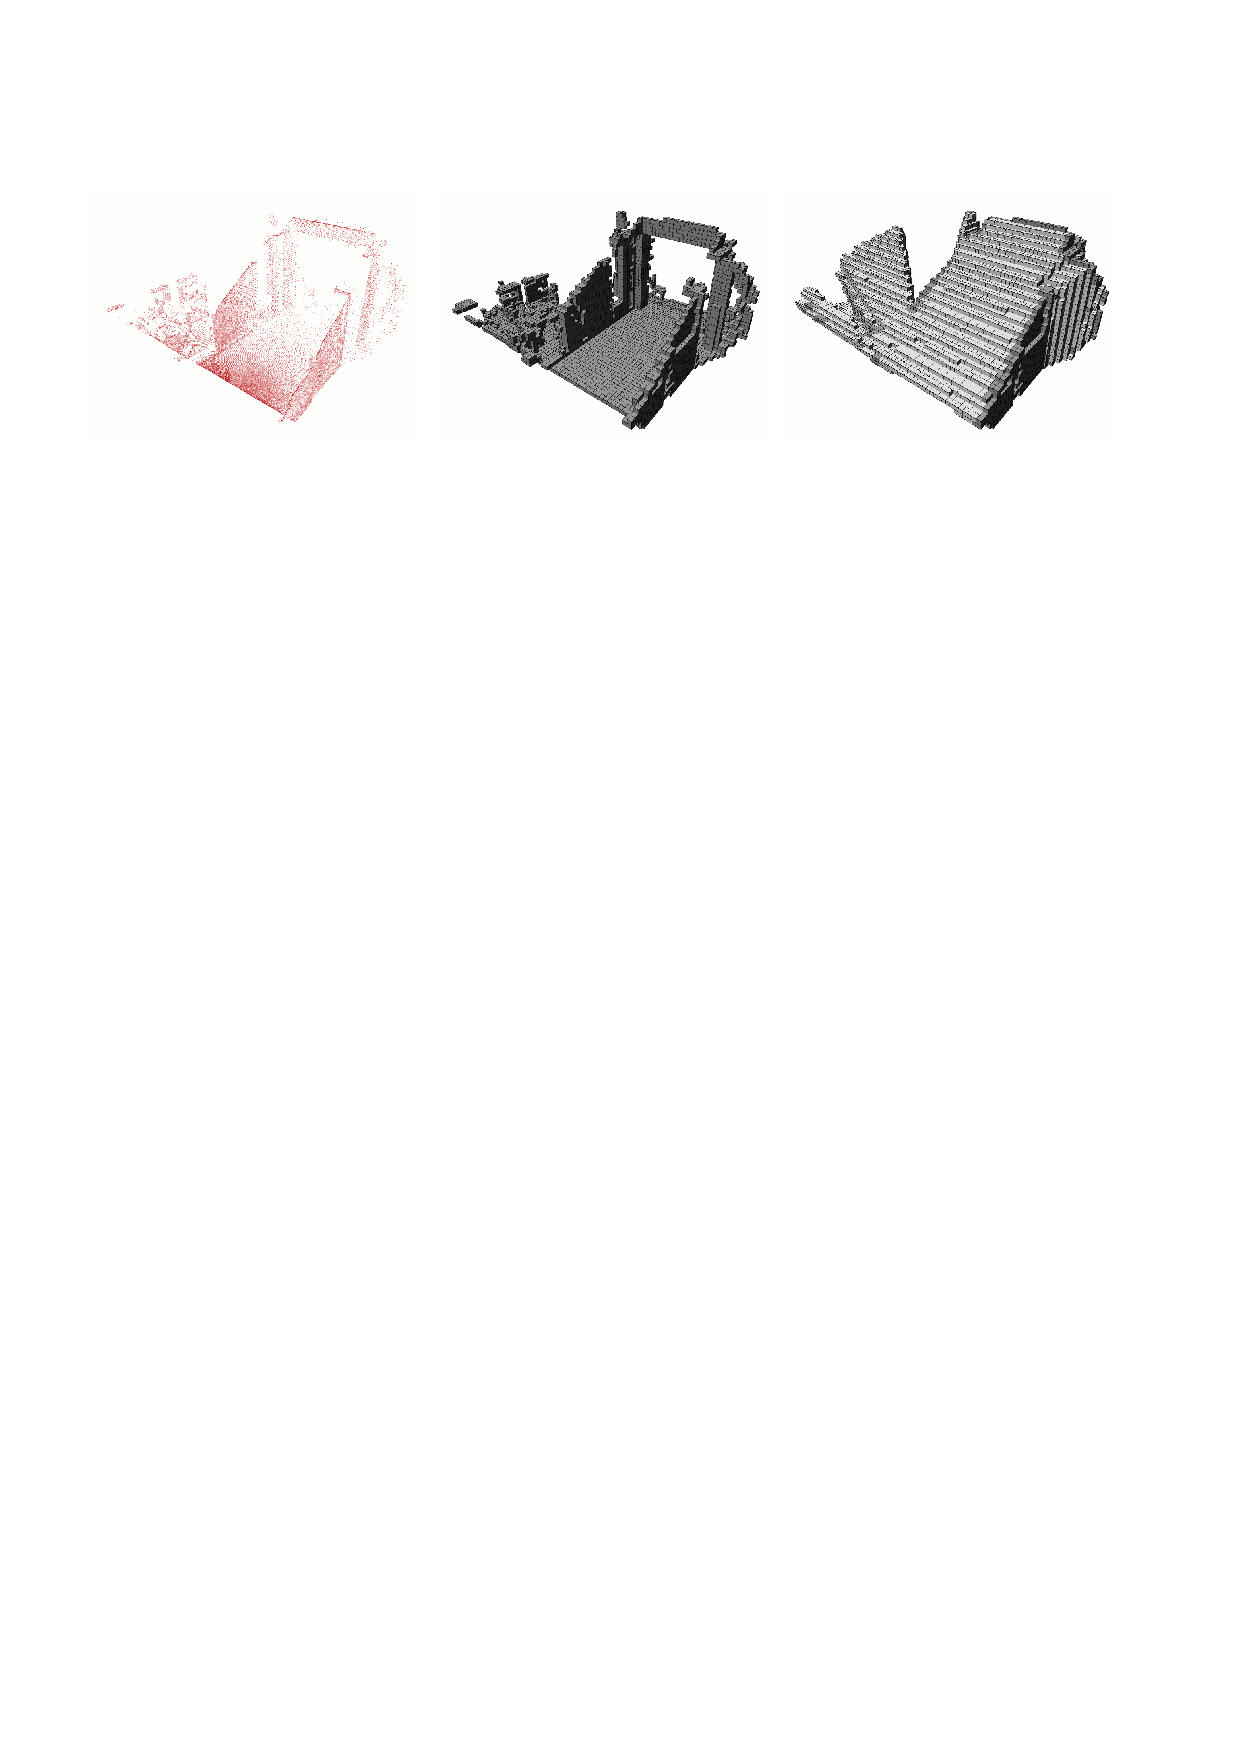
\includegraphics[width=0.95\textwidth]{figs/3d/free}
    \caption{\textit{Esquerda:} Representação do ambiente utilizando pointclouds e sem a possibilidade de se diferenciar espaços desconhecidos e vazios. \textit{Meio:} Representação em octomap com os espaços vazios omitidos. \textit{Direita:} Representação em octomap com os espaços vazios em cinza claros e os ocupados em cinza escuro.}
    \label{fig:free}
\end{figure}
\end{itemize}

\paragraph{Conclusão de análise técnica}\mbox{}\\
A representação 3D do ambiente a ser inspecionado por meio da utilização de Octomap se mostrou, além de mais eficiente no quesito de consumo de memória, perfeitamente alinhada com as necessidades particulares da solução a ser proposta. A possibilidade de busca e segmentação do mapa, possibilita a análise de partes isoladas do mapa e, consequentemente, a identificação de objetos esperados, assim como objetos estranhos e que não deveriam estar presentes. A diferenciação entre espaços vazios e cheios e a política de ocupância probabilística exercem uma função de segurança, a medida que explicitam qual parte do ambiente já foi inspecionada e atenuam possíveis ruídos externos e, também, intrínsecos ao sensor.

\subsection{Sistemas de potência}
Os sistemas de potência devem ser analisados tendo em vista a operação convencional e excepcional. Para a operação excepcional, é necessário o uso de cabo para o fornecimento de grande potência, sendo impossibilitado o uso de bateria para esta operação devido à potência de operação da bomba. Vale notar que a potência da bomba e a consequente espessura do cabo de alimentação é primordial para a definição do carretel para esta aplicação. 
Para operação convencional, há a possibilidade do uso de um outro carretel, independente do sistema de alimentação da bomba ou do uso de bateria e um sistema de comunicação por ultra-som.
 
\subsubsection{Carretel}
Carretéis industriais são dispositivos para recolhimento de cabos atuados por mola. Os cabos são fixados e conectados em contatos girantes.Tais dispositivos apresentam robustez estrutural e resistência ao tempo.
 
A partir da pesquisa realizada, é possível concluir que há boa disponibilidade de carretéis industriais para a aplicação visada, inclusive com graus de proteção adequados para umidade e resistência ao tempo (NEMA4) e perfil compacto. Vale notar, portanto, necessidades essenciais para a correta especificação e definição do produto:
\begin{itemize}
  \item O local disponível para fixação do carretel, calculando-se o comprimento ativo do cabo (a diferença de comprimento entre o cabo totalmente recolhido e o cabo totalmente não recolhido), o comprimento máximo suspenso do cabo e o comprimento máximo submerso do cabo.
  
  \item O tipo de cabo a ser utilizado, seu peso e resistência à tração, bem como o número de fios e o diâmetro deste. O número e espessura dos fios deve ser considerado não só pelo efeito deste no peso do cabo, mas também devido à necessidade dos contatos girantes para cada condutor
 
  \item A opção pelo uso de fibra ótica elimina a possibilidade de uso dos carretéis analisados, visto que não só há a questão de possíveis danos à fibra devido ao enrolamento do cabo como, principalmente, há a necessidade do uso de um acoplamento ótico girante, que não é disponibilizado nos carretéis analisados.
\end{itemize}
\paragraph{Conclusão de análise técnica}\mbox{}\\
 
Um carretel deve ser utilizado para alimentação da bomba, tendo em vista a operação excepcional. Um segundo carretel pode ser utilizado para alimentação e comunicação com o sistema eletrônico para operação convencional, tendo como alternativa o uso de um sistema de bateria e de comunicação por ultrassom.
 
\paragraph{Pesquisa de fornecedores}\mbox{}\\
Os fornecedores analisados que apresentam disponibilidade de carretéis adequados à aplicação visada são Cavotec e Conductix. Ambas as empresas apresentam representação no Brasil.
 
 
\subsubsection{Bateria}
 
Em relação às baterias, deve-se considerar sobretudo a densidade volumétrica de energia, já que o peso não é uma restrição tão significativa na aplicação visada.
Com a correta definição do tempo de operação e da tensão e corrente necessária para o sistema, podemos definir o tipo de bateria necessário.
Baterias de chumbo apresentam baixa densidade energética (aproximadamente 60 Wh/l) e auto-descarga em torno de 10 \% ao mês, são seguras e de fácil carga e descarga, mas têm sua vida útil significativamente reduzida devido a aumento de temperatura. Baterias de Ni-MH apresentam densidade de energia intermediária (aproximadamente 200Wh/l). As baterias de Ni-MH convencionais apresentam auto-descarga de cerca de 30 \% ao mês, tornando necessária a carga pouco tempo antes do uso, mas há a possibilidade de utilizar baterias de Ni-MH de baixa auto-descarga (Low Self Discharge), que apresentam menor densidade de energia, mas apresentam perdas inferiores a 2\% ao mês.
Finalmente, baterias de ion de lítio apresentam maior densidade de energia (aproximadamente 300Wh/l) e auto-descarga de cerca de 10\% ao mês, mas apresentam maior dificuldade de carga e a necessidade de dispositivos de proteção, apresentam perda de carga em temperaturas mais altas e questões de segurança.
Tendo em vista tais considerações, é razoável optarmos por baterias de Ni-Mh de baixa auto-descarga. Tais baterias não apresentam as preocupações de segurança das baterias de íon de lítio, simplificando os sistemas de carga e de proteção e são significativamente mais compactas que as baterias de chumbo.
\paragraph{Conclusão de análise técnica}\mbox{}\\
Tendo em vista a variedade de opções de baterias, podemos concluir que seu uso para a substituição de um segundo carretel será determinada pela disponibilidade e viabilidade do uso de um sistema de comunicação por ultrassom.